\section{Cluster-based Map Abstraction}
\label{aha:mapabstraction}
The annotated graph we have focused on creating to now is sufficient for a low-level search but inefficient for large problem sizes. 
Instead of planning every step, we would prefer to express a more general strategy using macro-operators.
We will achieve this by starting from the off-line decomposition technique described in \cite{botea04} and extending it to deal with large agents and multiple terrains. 
Our result from theorem {\ref{aha-theorem:reducibility} is key to the spatial abstraction described in this section. 
\par \indent
The general process in \cite{botea04} involves dividing a grid map into \emph{clusters}; subsets of the original grid map which result when the map is divided into a set of fixed-size square sections. Figure \ref{aha-fig:clustersandentrances}(a) shows the result of this decomposition approach; we use clusters of size 5 to split our toy map into 4 adjacent sections.
\par \indent
In the original work \emph{entrances} are obstacle-free transition areas of maximal size which exist along the border area between adjacent pairs of clusters. They are represented in the abstract graph by a pair of nodes connected by an undirected \emph{inter-edge} of weight 1.0. 
Our approach is similar but requires as a parameter $C$, the set of all capabilities. 
We thus begin by attempting to identify entrances $\forall c \in C$. 
\par \indent
We start at the beginning of the adjacent border area and extend the entrance until one of three termination conditions occurs: the end of the border area is reached, an obstacle is detected or the clearance value of nodes in either cluster begins to increase. 
The last condition is important to preserve completeness for our agents; just because a cluster can be reached does not guarantee that all locations within it are reachable. 
We thus identify all alternate-size entrances.
\par \indent
Once an entrance is found, we choose as the transition point the first pair of adjacent nodes which maximise clearance for $c$. 
This latter metric, $cv_{entrance}$ is computed by taking the minimum clearance among each node pair in the entrance area and selecting the largest value from the set. Thus, we add a new edge to the graph, $inter$ which we annotate $inter(c) = cv_{entrance}$. 
\par \indent
In figure \ref{aha-fig:clustersandentrances}(b) we present three entrances identified by scanning the border between clusters $c1$ and $c3$.
Entrances \emph{E1} and \emph{E2}, each of which span only part of the border area, are discovered using $\lbrace Ground \rbrace$ and $\lbrace Trees \rbrace$ capabilities. \emph{E3} meanwhile, which spans the whole border area, is discovered using the more complex $\lbrace Ground \vee Trees \rbrace$ capability. 
The connected tiles represent the locations of the subsequent transition points; the final result is shown in \ref{aha-fig:clustersandentrances}(c). 
Note that \emph{E1} and \emph{E3} are incident on the same pair of nodes in the abstract graph. This is due to our  strategy of actively attempting to re-use any existing nodes from the abstract graph. 
We thus produce an abstract \emph{multi-graph}.

\begin{figure}[htbp]
        \caption{\emph{Building clusters and identifying entrances} }
        \begin{center}
                        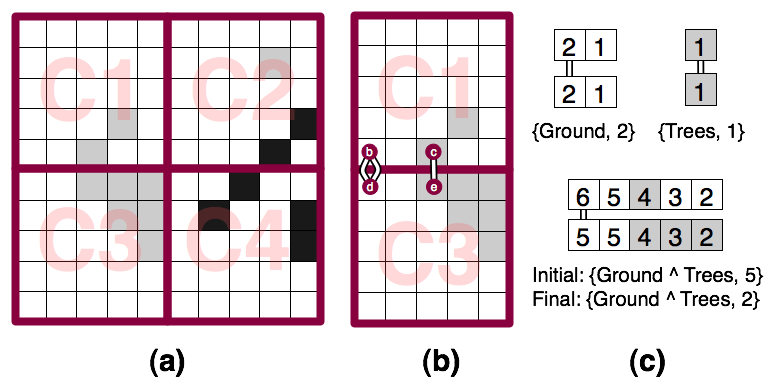
\includegraphics[scale=0.25]{diagrams/identifying_entrances.png}
        \end{center}
        \label{aha-fig:clustersandentrances}
\end{figure}

The final step in the decomposition involves attempting to add to the abstract graph a set of \emph{intra-edges} for each pair of abstract nodes inside a cluster. We achieve this by running multiple AA* searches $\forall (c, s) : c \in C, s \in S$.
\par \indent
Once a path is found we annotate the new edge, $intra$, with the capability and clearance parameters used by AA* and set its weight equal to the cost of the path. The algorithm terminates when all clusters have been considered. 
We term the resultant abstraction $initial$ and give the following lemmas to characterise its space complexity:

\input abstractionproperties
